\documentclass{template}
\usepackage{color}
\usepackage[hyphens]{url}
\usepackage{longtable}
\usepackage{graphicx}
\usepackage{enumitem}
\usepackage{pdfpages}
\usepackage{hyperref}

\def\etal{{\it et al.~}}
\newenvironment{packed_enum}{
\begin{enumerate}
  \setlength{\itemsep}{1pt}
  \setlength{\parskip}{0pt}
  \setlength{\parsep}{0pt}
}{\end{enumerate}}
\newenvironment{packed_item}{
\begin{itemize}
  \setlength{\itemsep}{1pt}
  \setlength{\parskip}{0pt}
  \setlength{\parsep}{0pt}
}{\end{itemize}}

\begin{document}

\title{Tor's Usability for Censorship Circumvention}
\numberofauthors{1}
\author{
 \alignauthor David Fifield\textsuperscript{1} and Linda N. Lee\textsuperscript{1}, Serge Egelman\textsuperscript{1,2}, David Wagner\textsuperscript{1}\\
   \vspace{0.5em}
   \affaddr{\textsuperscript{1}University of California, Berkeley, \{fifield,lnl,egelman,daw\}@cs.berkeley.edu}, \\
   \affaddr{\textsuperscript{2}International Computer Science Institute, egelman@icsi.berkeley.edu}\\
}
\maketitle

\begin{abstract}
{\color{red}
Tor has grown beyond its original purpose as and has 
since become an important Internet circumvention tool.
We specifically examine it usability as a censorship circumvention tool,
an essential facet for adoption and use.  
We focus our analysis on the connection configuration dialog of Tor browser,
as censorship circumvention requires correct transport configurations.
Our talk will describe a future study aimed at evaluating 
if and how easily users can circumvent censorship using Tor Browser,
isolating specific browser features to study in the process. 
To this end, we will conduct a large-scale user study examining hundreds of users 
on how they navigate Tor's configuration wizard to complete seven browsing tasks 
in three different adversarial settings. 
We solicit feedback to improve our study's design.}
\end{abstract}

\keywords{Censorship, Security, User Studies, Anonymity, Tor}

\section{Tor's Usability}
{\color {red}
%Idea is to cover background on Tor's usability as an anonymity tool, and then highlight the shift in focus to evaluating Tor's usability as a censorship circumvention tool. 

Tor is the most widely used anonymity tool today. However, there are complaints that Tor is not usable. Norcie~\cite{norcie2012eliminating} did an experiment which identified stopping points in Tor browser, 
finding out when people would get frustrated with Tor so much they would stop using it. 
%redo this next couple sentences into something better
But what about the people who are using Tor? what usability issues would there be if people were not stopped? 
To our knowledge, that has been the only user study of Tor. 
Since then, Tor has had a lot of updates. 
Additionally, there were a lot of features that were untested. 
There have been been no major usability evaluations of
Tor Browser since the introduction of the 4.0 series,
which introduced radical UI changes.

We briefly describe the results of a completed study
that examined the download and installation processes, 
as well as basic browsing behaviors.
This study uncovered a number of bugs and stopping points
which has already effected concrete change in the browser.

We ran a small pilot study of five journalists which involved a cognitive walk through in which 
participants explained the motivation for their actions and any confusion that they had during the process. 
We did this to find new stopping points, and sources of confusion. 
But in the process, we were also able to observe how users would download Tor, 
if they could understand the address bar/menu, how well they were able to complete basic tasks
(searching, setting new circuits, etc.), and generally if they had any usability complaints about the browser. 

We recruited five journalists from Berkeley by reaching out to journalist contacts. 
%Demographics here. 
During the study, we made a video recording of each participant's computer screen
and simultaneously projected it
into another room with Tor developers.
We recorded what they were saying out loud in their cognitive walk through,
and later added these words to the screen videos as subtitles.
The participants also took an exit survey which estimated their familiarity with technology and security. On average, participants took 26 minutes to complete the study ($\sigma = 7$~min).  The result was that people did have difficulty with installing Tor Browser (principally because of the Gatekeeper code-signing feature on OS~X), did not understand what many of the many options meant, and were confused about why certain things were happening. 
Our talk will feature brief highlights of the screen videos and a summary of interface changes.

After our first  usability evaluation of Tor, it was clear to us that so many of the features had been left unevaluated---such as advanced web browsing tasks, the configuration menu, automatic updates, and identity and cookie management. 
%say something about how we resolved this somehow, and how it doesn't necessarily need our attention now
We found that the most effective way to resolve the problems encountered was more user guidance and interface remodeling rather than continued user observations.
%emphasize how we are aiming for new research, not new test cases for debugging an interface
Rather than selecting the features to study in isolation, 
we decided to focus on an important use case of Tor browser, censorship circumvention. 
%say something along the lines of ``x people are using it for this, and there's no work on it,'' 
%if there are stats on this type of thing.
To our knowledge, this is the first user study investigating the usability of Tor as a 
censorship circumvention tool, rather than an anonymity tool. }



\section{Design}

\noindent {\bfseries Overview}
{\color {red}
% test tor, test improvements, may do followups on demand, push changes.

%improve what is below:
For users to circumvent censorship in their resident countries, they will need to configure Tor to set up a proxy, bridge, or both. There is a configuration wizard to help guide users through setting up their connection, but our hypothesis is that the average user will not easily be able to configure Tor correctly in these adverse settings, as they require the user to provide IP addresses of proxies or bridges to use. The goal of our experiment is to see how successful users are at carrying out common browsing tasks in an adversarial setting using Tor.}\\

\begin{figure}[t]
  \centering
    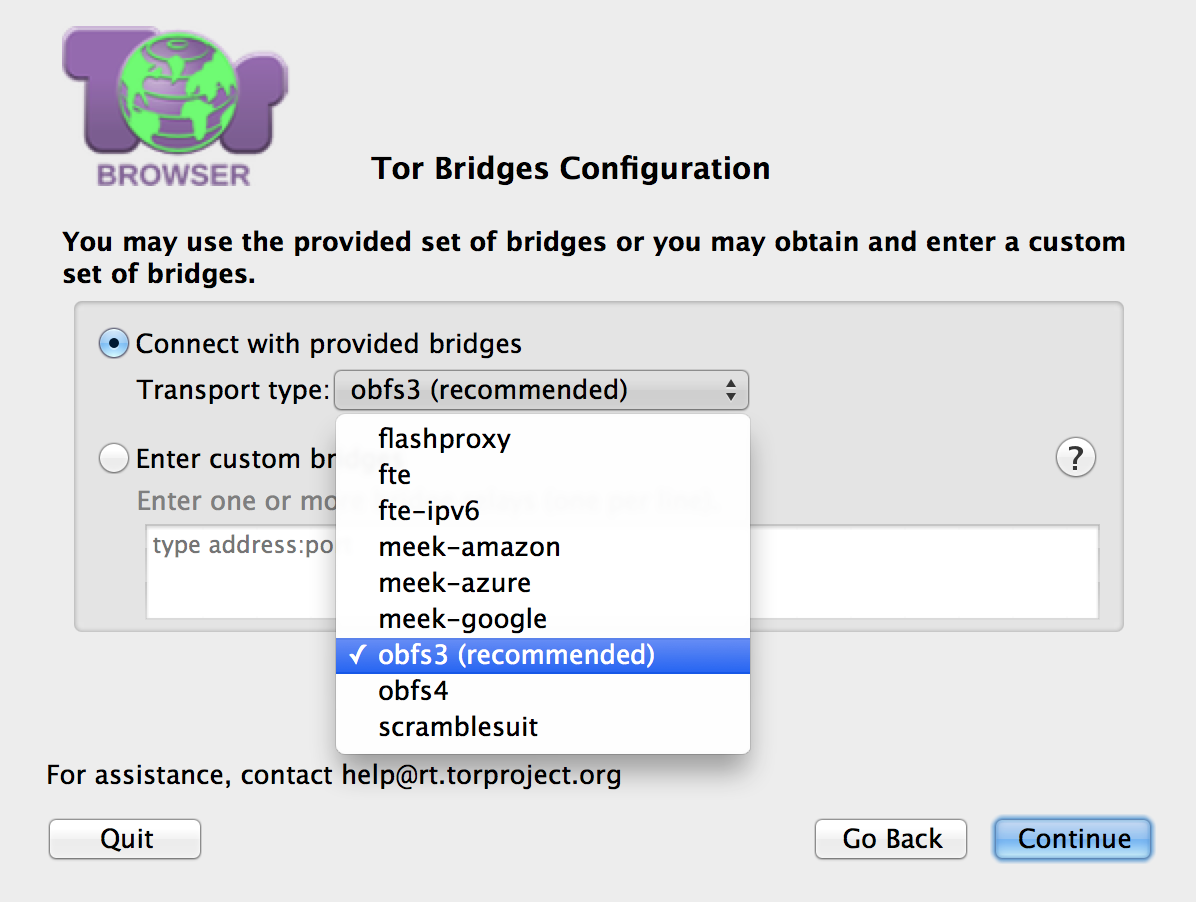
\includegraphics[width=0.5\textwidth]{configuration-screenshot.png}
    \caption{The Tor Bridges Configuration window of the Tor configuration interface. Tor users in censored environments and some of our participants will be required to select the correct bridge for circumventing censorship. Note that the interface prompts users to choose a transport type, which can be the source of confusion. Bridges are non-listed guard relays to the Tor network, and some of them can have transport types which obfuscate traffic in different ways.}
\end{figure}


\noindent {\bfseries Experiment Logistics} 
The IRB protocol to run this user study has been approved (2014-12-6995). 
We plan to recruit from 100-200 users for the purpose of this study, 
making it largest user study to examine Tor.  This study will be conducted at the 
Experimental Social Science Laboratory (Xlab)
at the University of California, Berkeley, which consists of 36 laptops with 
cubicle walls separating each laptop. We will use individual host firewalls to simulate
censorship environments and will record computer screens to capture 
user activity. The total length of the experiment, including briefing, completing the censorship 
circumvention tasks, exit survey, and debriefing, will take about an hour. 
Participants will be compensated \$30 for their time, which is more to cover 
minimum wage for an hour and any transportation costs to the lab.  \\

\noindent {\bfseries Experiment Flow} 
{\color {red}
% explain one experiment from start to end. 
At the start of the study, participants will be informed
of the role they they will be playing in the study. Particularly,
they will be informed that they are in a censorship environment
which prevents them from visiting certain websites, but they
are people who would like to visit those websites for 
leisurely purposes. 

%talk about how participants will be motivated to configure to 
%complete these tasks. participants will write down the answers 
%on a sheet of paper... 

We start off the experiment by telling them that they are in an adversarial setting, and that some websites are blocked and some websites are not. We will instruct them to visit notblocked.com and also blocked.com to illustrate the situation that they are in. We will also explain what Tor is, and how they can use it if necessary, and ask them to complete the set of tasks. To complete all the tasks, the participants will ultimately need to get the correct configuration settings for the country they are simulated to be in. We will end the experiment with a survey which asks them things like their security background, tech exposure, what was unexpected, what was hard, etc. We plan to analyze: which configuration tasks are hard (bridges versus proxies, etc.), how many were successful, how long it took users to configure, if they understood the process, if they were confident that it was working as expected, etc.} \\

\noindent {\bfseries Censorship Environment Simulation} 
{\color{red}
We plan to simulate three censorship environments.
They are informed by our experience with pluggable transports
and knowledge of commonly seen censorship techniques.
They are not meant perfectly to replicate the network environment
in any particular country; rather, they are abstract simulations
that are nevertheless inspired by reality.

% talk about how these censorship environments cover the UI path

\begin{itemize} \itemsep1pt \parskip0pt \parsep0pt
\item{Corporate network.}
A simulation of an enterprise or educational firewall.
Blocks all services but HTTP, HTTPS, and DNS.
Certain non-work-related domains, like youtube.com and torproject.org,
are blocked by DNS and HTTP inspection.
Blocked requests are redirected to a block page.
\item{DNS-only censor.}
This censor injects false replies to DNS queries
for forbidden domain names (DNS poisoning),
but does not do deep packet inspection on TCP streams.
Unlike the corporate censor, this censor allows protocols
outside a small whitelisted set.
\item{Comprehensive censor.}
Employs a variety of techniques, depending on the target.
May do DNS poisoning, IP blocking, and inspection of TCP streams
(examining the URL of HTTP requests, for example).
Some domains may be blocked by DNS and deep packet inspection;
others may additionally be blocked by IP address.
Tor relays are blocked by IP address.
Some domains, like wikipedia.org, may allow HTTP but not HTTPS.
Blocked requests fail silently (no block page).
\end{itemize}

In certain real censorship environment and our most 
prohibitive simulated censorship environments, only some of 
Tor's pluggable transports work in censorship environments
where others do not. Some of them require additional information
(like bridge addresses) before they work. Currently, we do not 
have a way to target test specific transports. However, we 
do ask why participants chose a specific pluggable 
transport in our exit survey to gain some insight.}\\

\noindent {\bfseries List of Tasks} 
In our experimental setup, successful completion of 
these given tasks requires of correct configuration.
The difficulty of circumventing  censorship to visit the 
websites required for the tasks will vary on the 
simulated censorship environment. Since all participants will be given the 
same set of tasks, regardless of the censorship environment, 
the difficulty of completing the tasks remains constant assuming
correct configuration. The tasks themselves are not intended to
be challenging.

The tasks were initially inspired by the top Alexa sites, 
an indication of representative and relevant browsing behavior. 
From these, we selected sites which were commonly censored, 
but filtered tasks that would require a participant to reveal private information 
(such as login information) for ethical considerations. These tasks
were further refined after performing a pilot study of the experiment. 
We hope the tasks convey an example of how of a user might 
browse the Internet in a censored environment. 

\begin{itemize} \itemsep1pt \parskip0pt \parsep0pt
\item Google search for the population of Zimbabwe. 
\item On Youtube, find a video playing Bach's ``Ode to Joy.'' 
\item Find the Amazon best-sellers in ``Movies \& TV.''
\item On Yahoo, find the exchange rate of dollars to euros.
\item Find the Wikipedia ``History'' portal's featured article. 
\item On Twitter, find the currently trending topics.
\item On Bing Maps, find directions from Time Square to Carnegie Hall.
\end{itemize}

\section{What we hope to accomplish}

We plan to finish the user study by the end of the semester. 
From this experiment, we hope to accomplish the following: 

\begin{itemize} \itemsep1pt \parskip0pt \parsep0pt
\item {\bfseries Test the Tor configuration interface} We will perform the largest-scale user study 
of Tor to date, measuring how users configure Tor in three different adversarial settings. 
\item {\bfseries Test an improved configuration interface} With the measurements collected
from testing the interface as-is, Nathan will be designing ways to improve the interface to minimize
time taken, paths taken, and error states reached.
\item {\bfseries Test an alternative configuration interface} A Tor developer has offered
to design a mock-up interface for an alternative configuration interface which will
greatly automate the process. There are tradeoffs between ease of use and transparency
of the system's, and ethical considerations with loggable errors resulting from automated configuration. 
\item {\bfseries Push changes} We have the support of Tor developers
to improve this interface. Additionally, since the configuration interface does not require 
any changes to the Tor Browser functionality, improvements to the interface will
be easy to deploy. 
\end{itemize}

\section{Resources}
\noindent Our online artifacts of the work done during this class, Fall 2015,
are below: 
\begin{itemize} \itemsep1pt \parskip0pt \parsep0pt
\item \href{https://github.com/lindanlee/circumvention-ux-tor}{github repo with experiment plans, code, and paper}
\item \href {https://github.com/lindanlee/circumvention-ux-tor/blob/master/pilot/1-strict.mp4}{pilot video 1}
	\href{https://github.com/lindanlee/circumvention-ux-tor/blob/master/pilot/2-lax.mp4}{pilot video 2}
\item \href{https://github.com/lindanlee/circumvention-ux-tor/blob/master/setup/setup-environment}{experimental setup code: firewall and screen capture} 
\item \href{https://github.com/lindanlee/circumvention-ux-tor/blob/master/setup/takedown-environment}{experimental takedown code: saving files and cleanup} 
\end{itemize}

%%  FROM ANONYMITY UX STUDY 
Our online artifacts of study of Tor as an anonymity tool, such as 
the summary, results, and resulting browser changes are below:
\begin{itemize} \itemsep1pt \parskip0pt \parsep0pt
\item \href{https://trac.torproject.org/projects/tor/wiki/org/meetings/2015UXsprint}{blog post summary}
\item \href{https://blog.torproject.org/blog/ux-sprint-2015-wrapup}{changes made to Tor}
\item \href{https://people.torproject.org/~dcf/uxsprint2015/}{subtitled screen videos}
\end{itemize}

\bibliographystyle{abbrv}
\bibliography{circumvention-experiment.bib} 
\end{document}
